% COVID-19-related disruptions in health services and data
% (c) 2023 Malcolm Gillies <malcolm.gillies@unsw.edu.au>
% https://github.com/mbg-unsw/pandemic-data-disruption
%
% This work is licensed under a
% Creative Commons Attribution-NonCommercial-ShareAlike 4.0
% International Licence
\documentclass[aspectratio=169,12pt]{beamer} % XXXX fix AR here
\usepackage[latin1]{inputenc}
\usepackage[T1]{fontenc}
\usepackage{textcomp}
\usefonttheme{serif} % need this with Charter font
\usetheme{Berlin}  % using default now
\usecolortheme{beaver}  % using default now
\usepackage[libertine]{libertine} % not using osf (old-style figures)
\usepackage[scale=0.9]{tgheros} % scale to match libertine
\usepackage[varqu,varl]{inconsolata}
\usepackage[libertine]{newtxmath}
\usepackage{graphicx}
\usepackage{tikz}
\usepackage{tikzpagenodes}
\usepackage{natbib}
\usepackage{gitinfo2}

\renewcommand{\gitMark}{\color{gray}\texttt{\tiny\gitBranch\,@\,\gitAbbrevHash\,\gitAuthorDate}}

\setbeamertemplate{navigation symbols}{} % remove navigation symbols
\setbeamercolor*{item}{fg=darkred}

\title{COVID-19-related disruptions in health services and data: Tracing causes and effects}
\author{Malcolm Gillies <malcolm.gillies@unsw.edu.au>}
\date{27 April 2023}
\usebackgroundtemplate{%
\begin{tikzpicture}[remember picture,overlay]
    \node[anchor=south west,scale=1,rotate=90] at ([shift={(0cm,0cm)}]current page marginpar area.south east) {\gitMark};
\end{tikzpicture}%
}
\begin{document}

{
%\usebackgroundtemplate{}
\begin{frame}
\titlepage
\end{frame}
}

\begin{frame}{Background: Human behaviour c. March 2020}
\centering

\includegraphics[height=0.75\textheight]
	{ref/toilet-paper-crop.jpg}

	\tiny 9 March 2020

	\copyright\: Christopher Corneschi.
	Reproduced under CC-BY-SA licence [cropped from original]
	% XXXX nice to rotate this and put on the right
\end{frame}

\begin{frame}{Background: Google mobility data, Sydney, 2020}
\centering
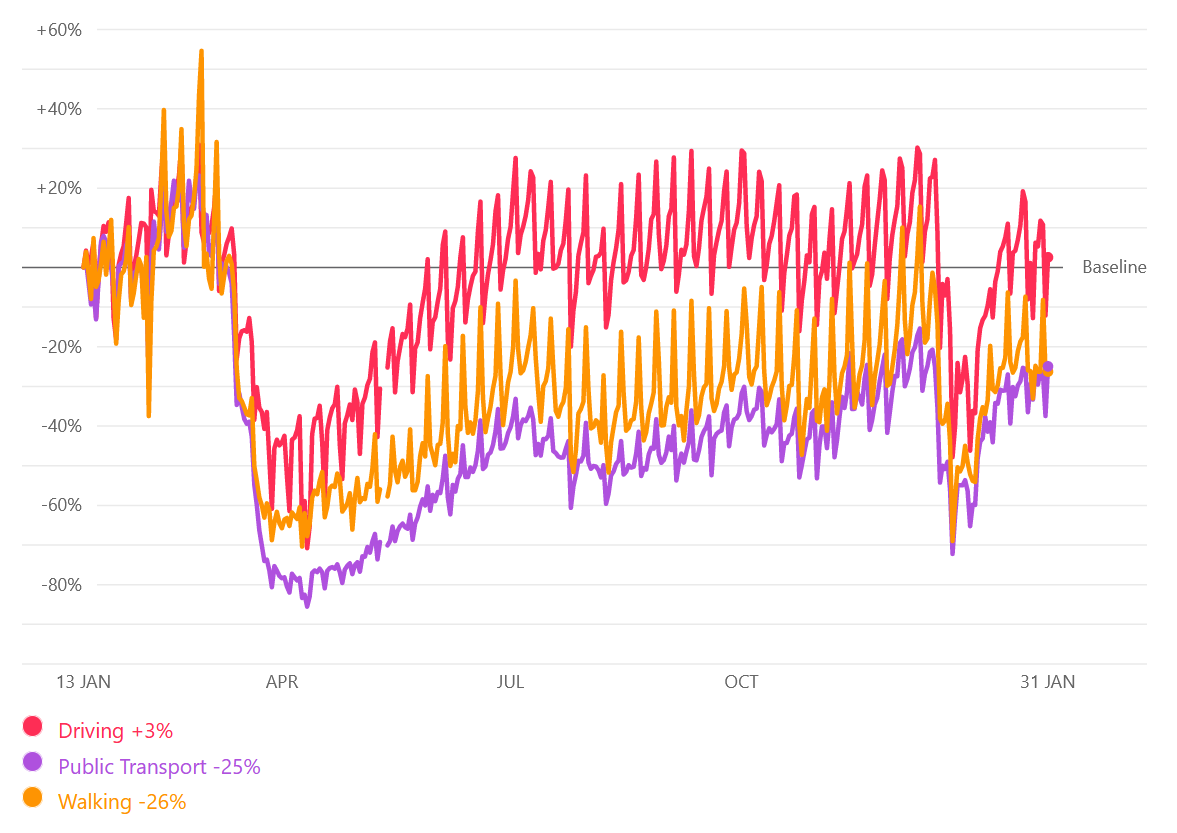
\includegraphics[height=0.8\textheight]
        {ref/google-mobility-20210202.PNG}
% https://covid19.apple.com/mobility
\end{frame}

\begin{frame}{Results: Changes in primary care consultation rates}
\centering
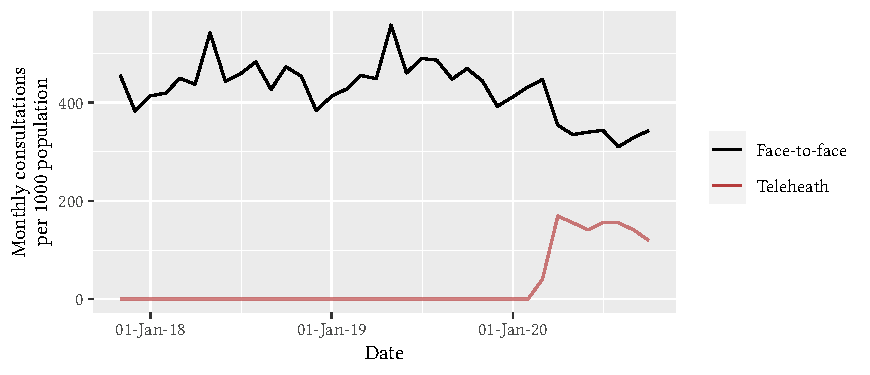
\includegraphics{ref/latex-suppmbs-1.pdf}
\end{frame}

\begin{frame}{Results: Changes in antibiotic dispensing}
\centering
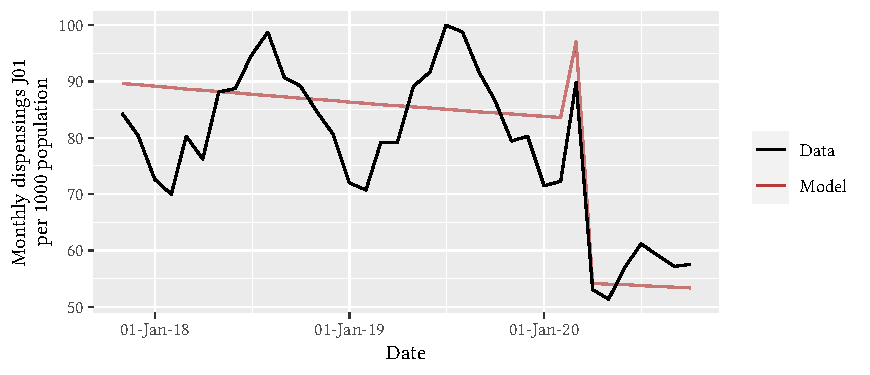
\includegraphics{ref/latex-j01armap3-1.pdf}
\end{frame}

\begin{frame}{Results: Top 10 antibiotics step changes}
\centering
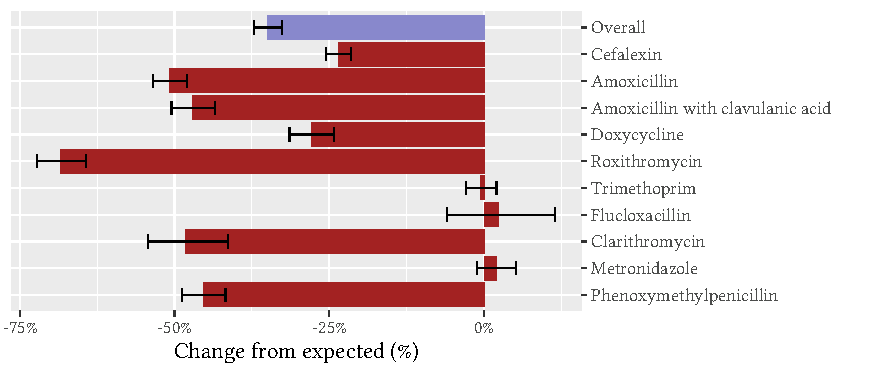
\includegraphics{ref/latex-j01arimatab-1.pdf}
\end{frame}

\begin{frame}{Results: Antibiotic changes by prescriber specialty}
\centering
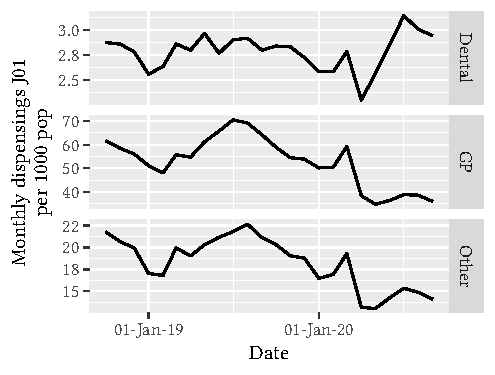
\includegraphics{ref/latex-j01specialty-1.pdf}
\end{frame}

\begin{frame}{ABS Estimated Resident Population: Projected vs Reported 1}
	\center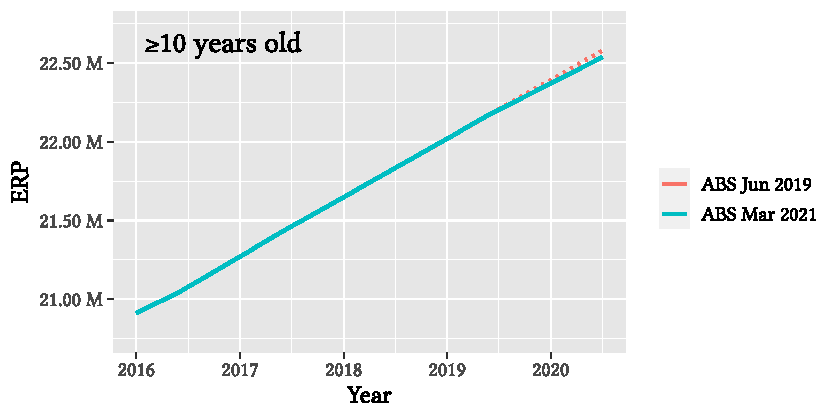
\includegraphics[height=0.75\textheight]{ref/pops-overall.pdf}
	\begin{flushright}\tiny\texttt{\url{https://www.abs.gov.au/statistics/people/population/national-state-and-territory-population}}\end{flushright}
\end{frame}

\begin{frame}{ABS Estimated Resident Population: Projected vs Reported 2}
	\center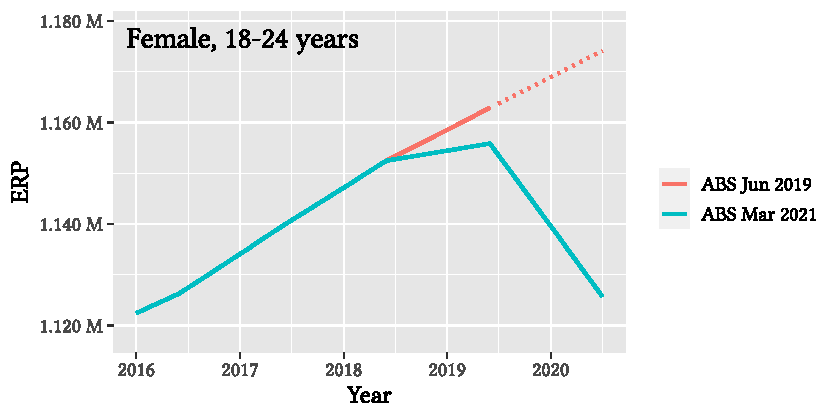
\includegraphics[height=0.75\textheight]{ref/pops-f18-24.pdf}
	\begin{flushright}\tiny\texttt{\url{https://www.abs.gov.au/statistics/people/population/national-state-and-territory-population}}\end{flushright}
\end{frame}

\begin{frame}{ABS components of population growth}

	\center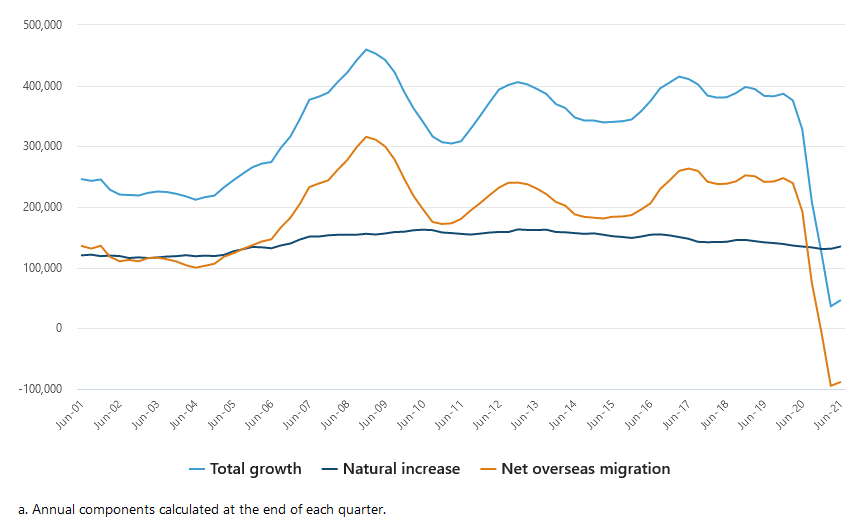
\includegraphics[height=0.75\textheight]{ref/pop-components.PNG}
	\begin{flushright}\tiny\texttt{\url{https://www.abs.gov.au/statistics/people/population/national-state-and-territory-population}}\end{flushright}
\end{frame}

\begin{frame}{Net overseas migration: PBS/MBS eligibility?}
	\center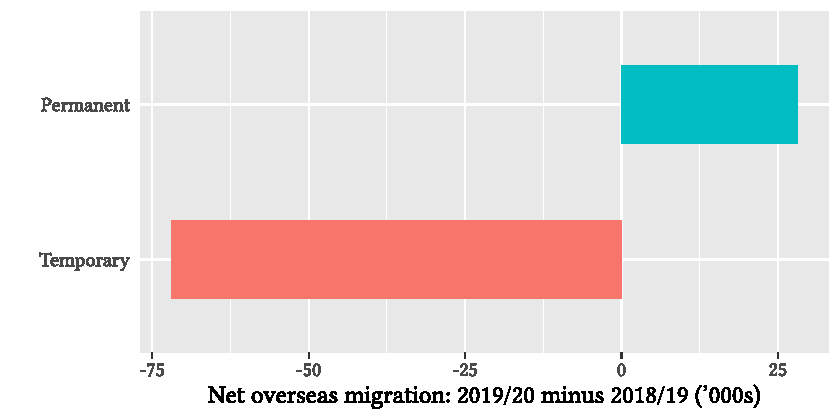
\includegraphics[height=0.75\textheight]{ref/pops-nom.pdf}
	\begin{flushright}\tiny\texttt{\url{https://www.abs.gov.au/statistics/people/population/migration-australia/latest-release}}\end{flushright}
\end{frame}

\begin{frame}{Finally}
	\begin{itemize}
		\item Remember they're \emph{estimated} resident populations
		\item As 2021 census results become available, 2017--2020 will be adjusted
	\end{itemize}
\end{frame}

\begin{frame}{Thanks}
    \begin{itemize}
        \item Australian Government Services Australia for providing the data
	\item Andrea
	\item MIRP crew
	\item Melisa Litchfield for assisting with data access and ethics approval
    \end{itemize}
\vfill
	Published in \emph{Br J Clin Pharmacol} 2021 doi:\href{https://doi.org/10.1111/bcp.15000}{10.1111/bcp.15000}
\end{frame}

\begin{frame}{References}
%        \bibliographystyle{apalike}
%        \bibliographystyle{abbrv}
        \tiny\bibliography{pandemic-disruption.bib}
        \bibliographystyle{abbrvnat}
\end{frame}

\end{document}
